\section{Czym się zajmowałem}
Zajmowałem się implementacją i rozwijaniem back-endu kompilatora, to jest klas Lexer i Parser. Wiązało się to z badaniem możliwości i ograniczeń biblioteki pyparsing.

Utrzymywałem też dokumentację składni języka w EBNF.

Ze względu na ograniczenia czasowe projektu nie udało się zaimplementować kilku elementów, których zrealizowanie zakładano w początkowej fazie projektu, takich jak obsługa różnych systemów liczbowych do reprezentacji liczb czy definiowanie złożonych właściwości.

\section{Tokeny}
Przy wyborze tokenów staraliśmy się zachować zgodność ze sposobem zapisu atrybutów i operacji w UMLu (stosowanie oznaczeń '-', '+', etc. w przypadku widoczności) i ułatwić zrozumienie kodu (w przypadku ograniczeń: użycie wyrazów angielskich 'allow', 'require').


\section{Produkcje}
Na diagramach składni tokeny wyróżniono ciemniejszym kolorem. Elementy należące do biblioteki pyparsing wyróżniono czarnym kolorem.

\subsection{Obiekty}
\begin{itemize}
\item grammar:

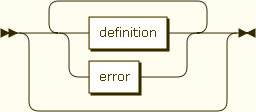
\includegraphics[scale=0.66]{images/grammar/grammar.png}

\item definition:

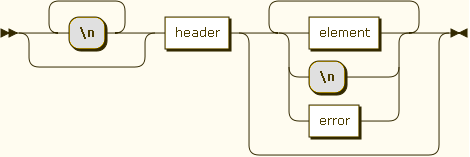
\includegraphics[scale=0.66]{images/grammar/definition.png}

\item header:

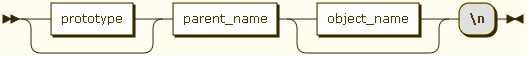
\includegraphics[scale=0.66]{images/grammar/header.png}

\item parent\_name:

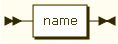
\includegraphics[scale=0.66]{images/grammar/name_xx.png}

\item object\_name:

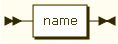
\includegraphics[scale=0.66]{images/grammar/name_xx.png}

\item element:

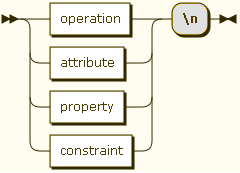
\includegraphics[scale=0.66]{images/grammar/element.png}
\end{itemize}
\subsection{Atrybuty}
\begin{itemize}
\item attribute:

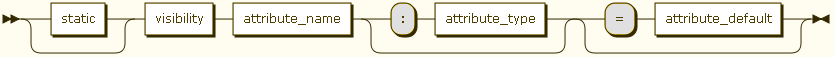
\includegraphics[scale=0.66]{images/grammar/attribute.png}

\item attribute\_name:

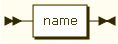
\includegraphics[scale=0.66]{images/grammar/name_xx.png}

\item attribute\_type:

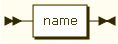
\includegraphics[scale=0.66]{images/grammar/name_xx.png}

\item attribute\_value:

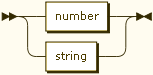
\includegraphics[scale=0.66]{images/grammar/attribute_value.png}
\end{itemize}
\subsection{Operacje}
\begin{itemize}
\item operation:

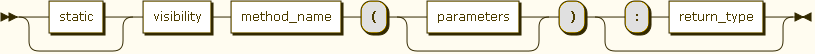
\includegraphics[scale=0.66]{images/grammar/operation.png}

\item operation\_name:

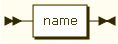
\includegraphics[scale=0.66]{images/grammar/name_xx.png}

\item return\_type:

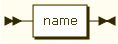
\includegraphics[scale=0.66]{images/grammar/name_xx.png}

\item parameters:

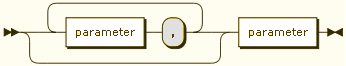
\includegraphics[scale=0.66]{images/grammar/parameters.png}

\item parameter:

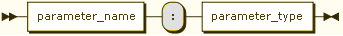
\includegraphics[scale=0.66]{images/grammar/parameter.png}

\item parameter\_name:

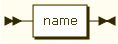
\includegraphics[scale=0.66]{images/grammar/name_xx.png}

\item parameter\_type:

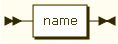
\includegraphics[scale=0.66]{images/grammar/name_xx.png}
\end{itemize}
\subsection{Właściwości}
\begin{itemize}
\item property:

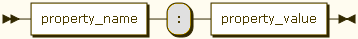
\includegraphics[scale=0.66]{images/grammar/property.png}

\item property\_name:

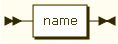
\includegraphics[scale=0.66]{images/grammar/name_xx.png}

\item property\_value:

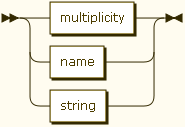
\includegraphics[scale=0.66]{images/grammar/property_value.png}
\end{itemize}
\subsection{Ograniczenia}
\begin{itemize}
\item constraint:

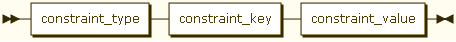
\includegraphics[scale=0.66]{images/grammar/constraint.png}

\item constraint\_type:

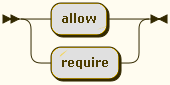
\includegraphics[scale=0.66]{images/grammar/constraint_type.png}

\item constraint\_key:

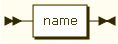
\includegraphics[scale=0.66]{images/grammar/name_xx.png}

\item constraint\_value:

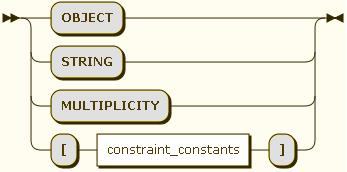
\includegraphics[scale=0.66]{images/grammar/constraint_value.png}

\item constraints\_constants:

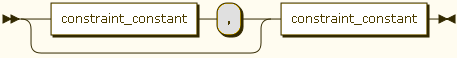
\includegraphics[scale=0.66]{images/grammar/constraint_constants.png}

\item constraint\_constant:

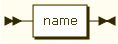
\includegraphics[scale=0.66]{images/grammar/name_xx.png}
\end{itemize}
\subsection{Generyczne}
\begin{itemize}
\item multiplicity:

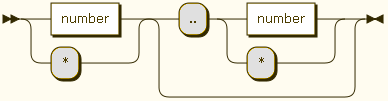
\includegraphics[scale=0.66]{images/grammar/multiplicity.png}

\item visibility:

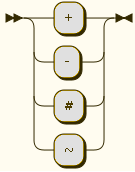
\includegraphics[scale=0.66]{images/grammar/visibility.png}

\item static:

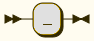
\includegraphics[scale=0.66]{images/grammar/static.png}

\item prototype:

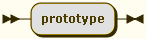
\includegraphics[scale=0.66]{images/grammar/prototype.png}

\item error:

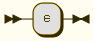
\includegraphics[scale=0.66]{images/grammar/error.png}
\end{itemize}
\subsection{pyparsing}
\begin{itemize}
\item number:

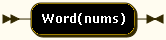
\includegraphics[scale=0.66]{images/grammar/number.png}

\item name:

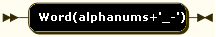
\includegraphics[scale=0.66]{images/grammar/name.png}

\item string:

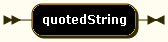
\includegraphics[scale=0.66]{images/grammar/string.png}
\end{itemize}

